%
% BUS 314: Resourcing New Ventures - A Course Overview
% Section: Financials
%
% Author: Jeffrey Leung
%

\section{Financials}
	\label{sec:financials}
\subsection{Basics}
	\label{subsec:financials:basics}
\begin{easylist}

& Measures:
	&& \textbf{Stock measure:} Current value held at a given time
	&& \textbf{Flow measure:} Change in a value over time

& \textbf{Liability:} Obligation to a creditor
& \textbf{Asset:} Tangible resource held
& \textbf{Equity:} Assets which may have liabilities attached
	&& Equation: Value of equity = assets - liabilities

& \textbf{Revenue/income:} Money generated
	&& \textbf{Sales/operating revenue:} Money generated from operations
	&& \textbf{Non-operating revenue:} Money generated which is not from an operation (e.g. investment interest)

& \textbf{Expense:} Money spent
	&& \textbf{Cost of Goods Sold (COGS):} Direct cost of production (e.g. materials, labor)
	&& \textbf{Non-manufacturing/Operating expense:} Expense not directly associated with productions (e.g. employee benefits)

& \textbf{Profit:} Difference between total revenue and total expenses

& \textbf{(Financial) capital:} Funds available to be used for production
	&& \textbf{Working capital:} Assets available to pay off liabilities (difference between total liabilities and total assets)

& \textbf{Accounts Receivable:} Revenues which are agreed but have not yet been received
	&& Are assets

\end{easylist}
\subsection{Balance and Income Sheet}
	\label{subsec:financials:balance-and-income-sheet}
\begin{easylist}

& \textbf{Balance sheet:} Stock measure which contains information about assets, liabilities, equity
	&& Represents the value of all assets and their method of financing (debt/equity) at a point in time
	&& Used to:
		&&& Examine liquidity
		&&& Determine financial flexibility
	&& Basis for return on equity/assets, DSO, inventory turnover, etc.
		&&& \textbf{Days Sales Outstanding (DSO):} Average number of days to collect payment after sale
			&&&& Ideal when low
	&& Total assets is equal to total liabilities plus stockholders' equity
	&& Example: See figure~\ref{img:balance-sheet-example}

\end{easylist}
\begin{figure}[!htb]
	\centering
	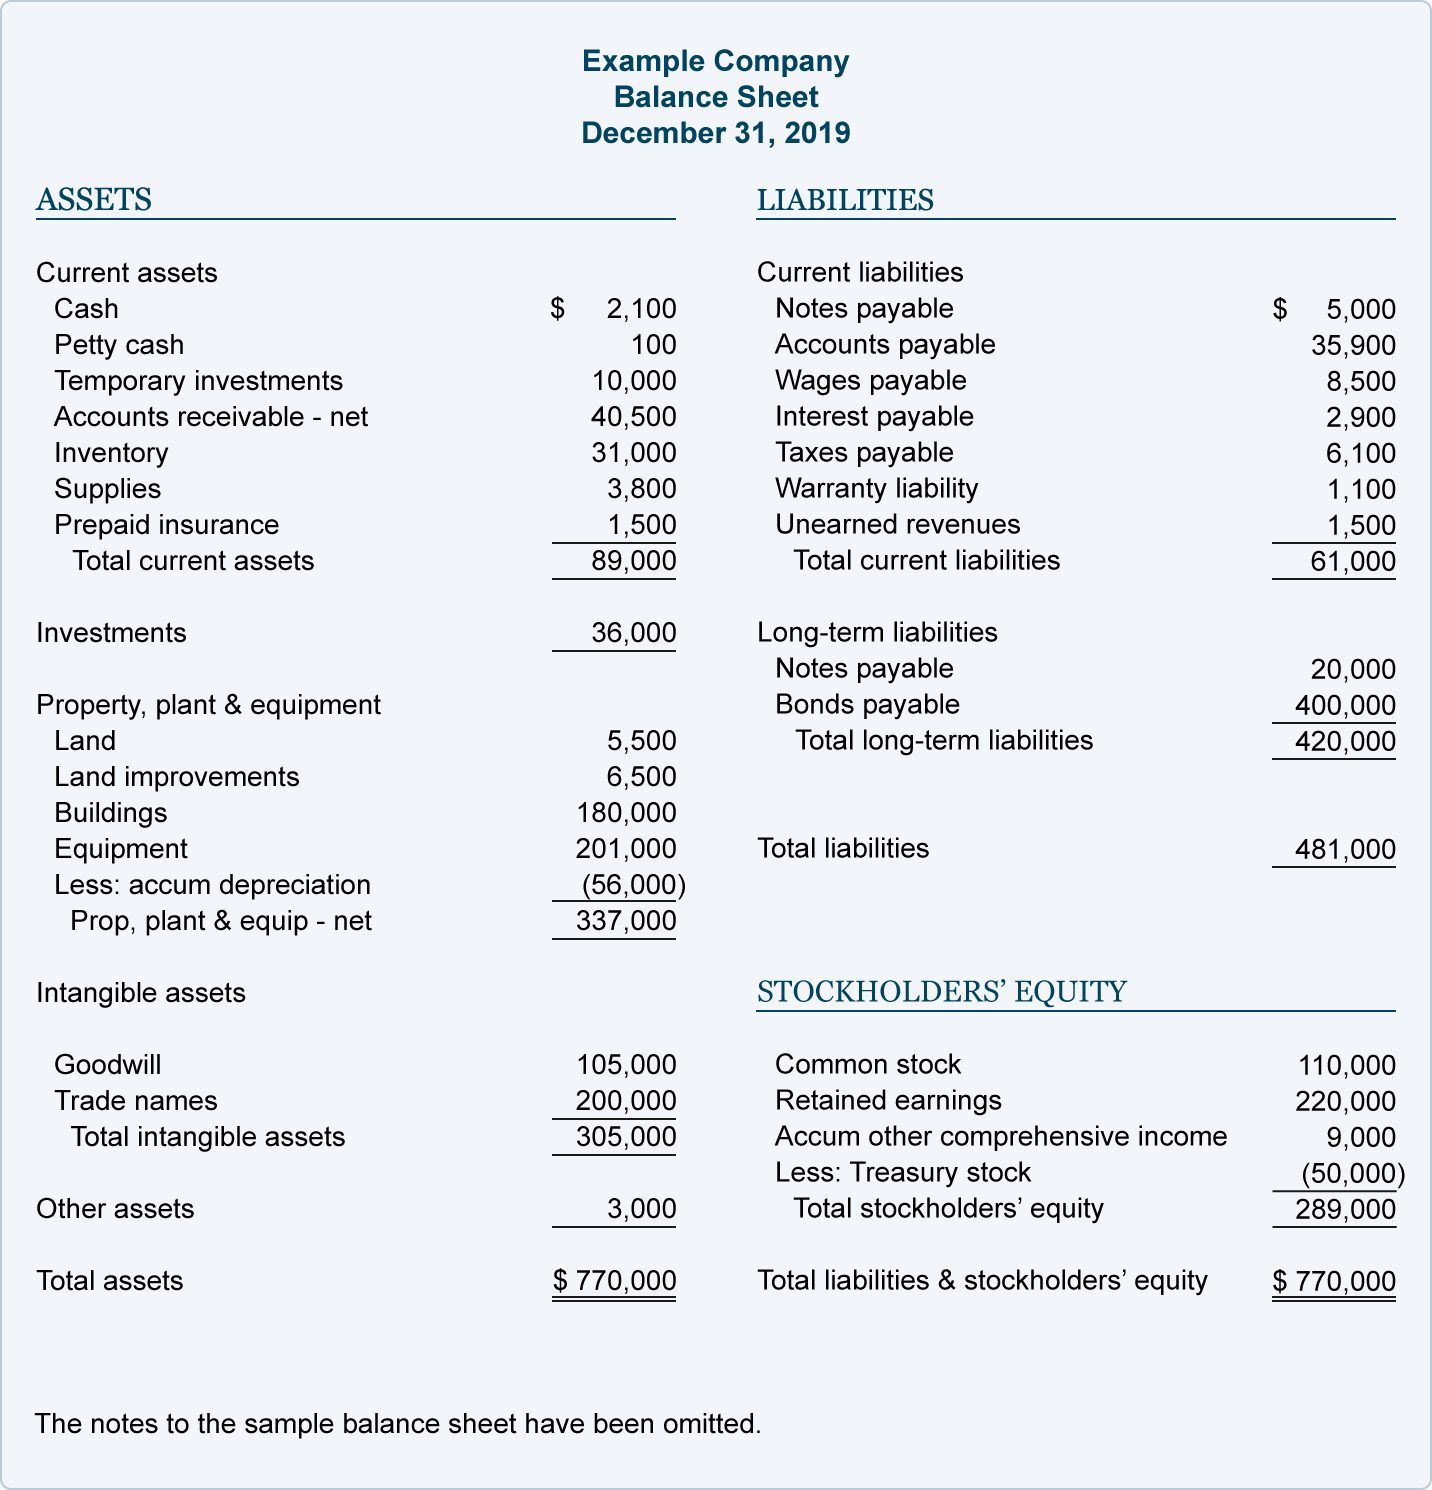
\includegraphics[width=.8\linewidth]{balance-sheet}
	\caption{Example of a Balance Sheet}
	\label{img:balance-sheet-example}
\end{figure}
\begin{easylist}

& \textbf{Income statement:} Flow measure which contains revenues, expenses, profit/income
	&& Represents the change in financial impact of operations over time
	&& Used to:
		&&& Evaluate past financial performance
		&&& Predict future cash flows
	&& Does not analyze:
		&&& Cash flow
		&&& Currently available funds
	&& Basis for gross/operating/net margin
	&& Example: See figure~\ref{img:income-statement-example}

\end{easylist}
\begin{figure}[!htb]
	\centering
	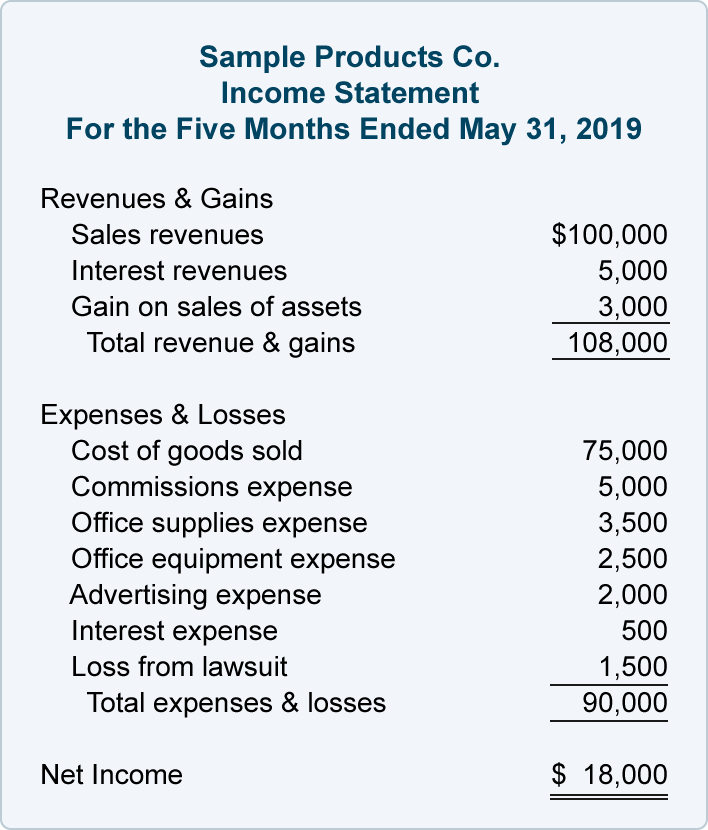
\includegraphics[width=.6\linewidth]{income-statement}
	\caption{Example of an Income Statement}
	\label{img:income-statement-example}
\end{figure}

\subsection{Financial Ratios}
	\label{subsec:financials:financial-ratios}
\begin{easylist}

& Categories of ratios:
	&& \textbf{Profitability ratio:} Proportional difference between profits over time or against other entities (e.g. gross vs. net margin)
	&& \textbf{Activity ratio:} Measure of efficiency of use of assets (e.g. DSO)
	&& \textbf{Liquidity ratio:} Measure of the ability to pay its liabilities when due (e.g. current ratio)
	&& \textbf{Coverage ratio:} Measure of the ability to meet financial obligations (e.g. months of cash burn in bank)

& Ratios:
	&& The greater, the better

	&& \textbf{Gross (profit) margin:} Difference measure which is the sales revenue minus cost of goods sold
		&&& Represents how efficiently a company creates its product

	&& \textbf{Operating margin:} Ratio measure which is (sales revenue minus operating costs) divided by sales revenue
		&&& Less than the gross margin
		&&& Represents how efficiently a company absorbs operating costs

	&& \textbf{Net (profit) margin:} Ratio measure which is net income divided by sales revenue
		&&& Less than the operating margin
		&&& Represents baseline of how much revenue per dollar is translated into profit

	&& \textbf{Return on assets:} Profitability measure which is (asset turnover times profit per asset)

\end{easylist}
\subsection{Cash Flow}
	\label{subsec:financials:cash-flow}
\begin{easylist}

& Consume cash when you:
	&& Increase assets (e.g. buying equipment)
	&& Decrease liabilities (e.g. paying back a loan, paying a supplier faster)
& Generate cash when you:
	&& Decrease assets (e.g. reducing inventory/accounts receivable)
	&& Increase liabilities (e.g. getting a loan)
	&& Issue equity (e.g. sell shares)
& No effect on cash when you:
	&& Change depreciation estimates

& \textbf{Cash flow statement:} Flow measure which contains operating, investing, and financing cash flow and the business activity which generated it
	&& For each line item, information contains: Source, amount, difference
	&& Example: See figure~\ref{img:cash-flow-statement-example}

\end{easylist}
\begin{figure}[!htb]
	\centering
	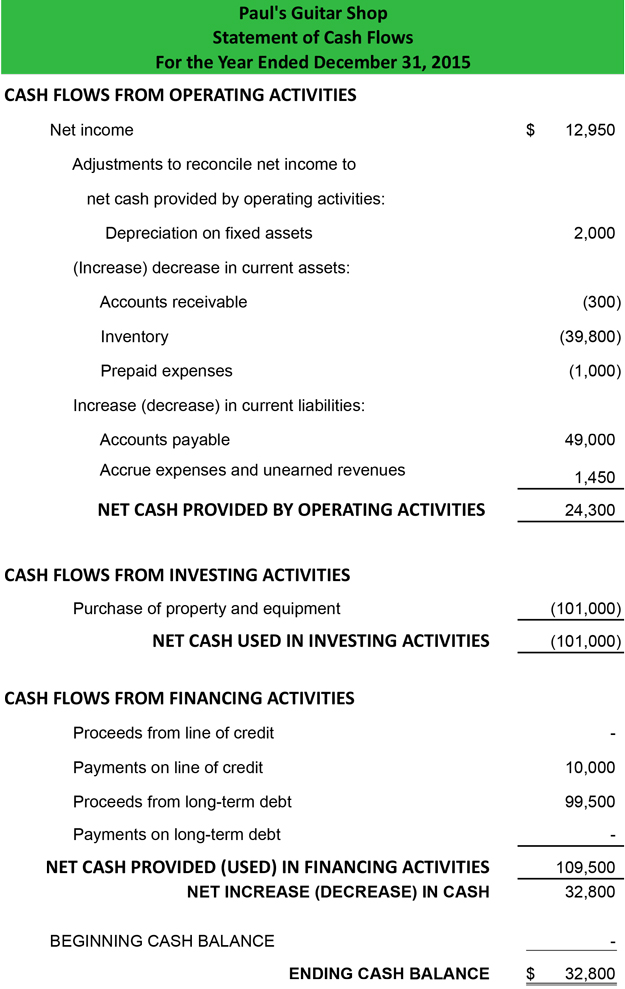
\includegraphics[width=.6\linewidth]{cash-flow-statement}
	\caption{Example of a Cash Flow Statement}
	\label{img:cash-flow-statement-example}
\end{figure}

\subsection{Balanced Scorecards}
	\label{subsec:financials:balanced-scorecards}
\begin{easylist}

& \textbf{Scorecard:} Perspective to view the health of an entity which has both a goal and an entity
	&& \textbf{Measure:} Method of quantifying a value
	&& \textbf{Goal:} Qualitative objective

& 4 scorecards:
	&& \textbf{Financial perspective:} Financial health
	&& \textbf{Customer perspective:} Customer interest and retention in the product
	&& \textbf{Internal business perspective:} Ability to efficiently and effectively deliver product
	&& \textbf{Learning/growth perspective:} Ability to innovate and continually create value

\end{easylist}
\subsection{Miscellaneous Concepts}
	\label{subsec:financials:miscellaneous-concepts}
\begin{easylist}

& Operating expenses do not include cost of goods sold

& \textbf{Insolvency/bankruptcy:} State where the value of the assets are less than the value of the liabilities

& Goodwill: Additional money paid in a purchase above valuation

& Profit can be manipulated by changing estimates/assumptions such as:
	&& Amortization of assets over longer/shorter periods of time
	&& Cpitalizing R\&D so it does not appear on the income statement

& \textbf{Unit economics:} Revenue or profit from one unit of a product/service
	&& Example of application: Number of units which must be sold to cover fixed costs
	&& Examples of metrics: Monthly active users (MAU), active revenue per user (ARPU)

& \textbf{Triple Buttom Line (3BL/TBL):} Measurement system across social, environmental, and financial aspects

\end{easylist}
\subsection{Equity}
	\label{subsec:financials:equity}
\begin{easylist}

& Multiple rounds of share distribution

& \textbf{Intellectual property:} Concept, knowledge, and technology which is the property of an entity (person, company, etc.)




\end{easylist}
\clearpage
